\chapter{Methodology}
As outlined in the introduction, we seek to find out if we can use consumer energy time series data to identify clusters of consumption patterns and can we use geographic and demographic data about those consumers to predict which cluster a consumer belongs to. In order to answer this question we're going to look at ways and methods to read in a large time series data file and perform clustering techniques to discover distinct groups based on energy consumption. We then will look at ways in which to use accompanying geographic and demographic data to classify a consumer into one of the distinct energy clusters.

\section{Description of Data}
    The data available was sourced from the UK Data Archive, Study Number 7591 - Energy Demand Research Project: Early Smart Meter Trials, 2007-2010. It contains the following:
    \subsection{Smart Meter Electrical Energy Consumption Readings}
        \subsubsection{Description of Variables}
    
            \\
            This file is in a CSV format. The electrical energy consumption file contains 413,836,038 readings in total for 14,621 households with a total disk space of 12GB. There are 4 variables, the description of each can be found in the accompanying documentation: 
        \begin{center}
            \begin{tabular}{|l | l|}
            \hline
             \textbf{Variable Name} & \textbf{Description} \\
             \hline\hline
             ANON\_ID & Integer case identifier (unique, not null, use to \\&  link records in the other files) \\ 
             \hline
             ADVANCEDATETIME & Date-Time of electricity read (half-hour precision) \\
             \hline
             HH & Half-hour indicator for each day (1-48) \\
             \hline
             ELECHKWH & Unit of kilowatt-hours consumed in that half-hour \\
             \hline
            \end{tabular}
        \end{center}
        
        \subsubsection{Exploratory Data Analysis on Consumption Data Set}
        Performing Exploratory Data Analysis (EDA) provides valuable insights, it introduces the data set and describes the data being studied. This data set contains the energy consumption measured by smart meters (in kilowatt-hours) starting at midnight and taking measurements every half-hour onwards. This is a classic example of a time-series data set with $key:value$ entries. Here our key is the time stamp at which a reading was taken (ADVANCEDATETIME) and the value is the consumption amount (ELECKWH). In addition to this we have the device identification (represented as ANON\_ID), we discuss how the data is to be structured in a future section, 3.3.2. This section will focus on carrying out EDA on a time period partition (or epoch) of the data set from the first 'chunk' of data which relates to the first 100,000 entries in the data set. 
        
        \begin{figure}[H]
        \centering     
        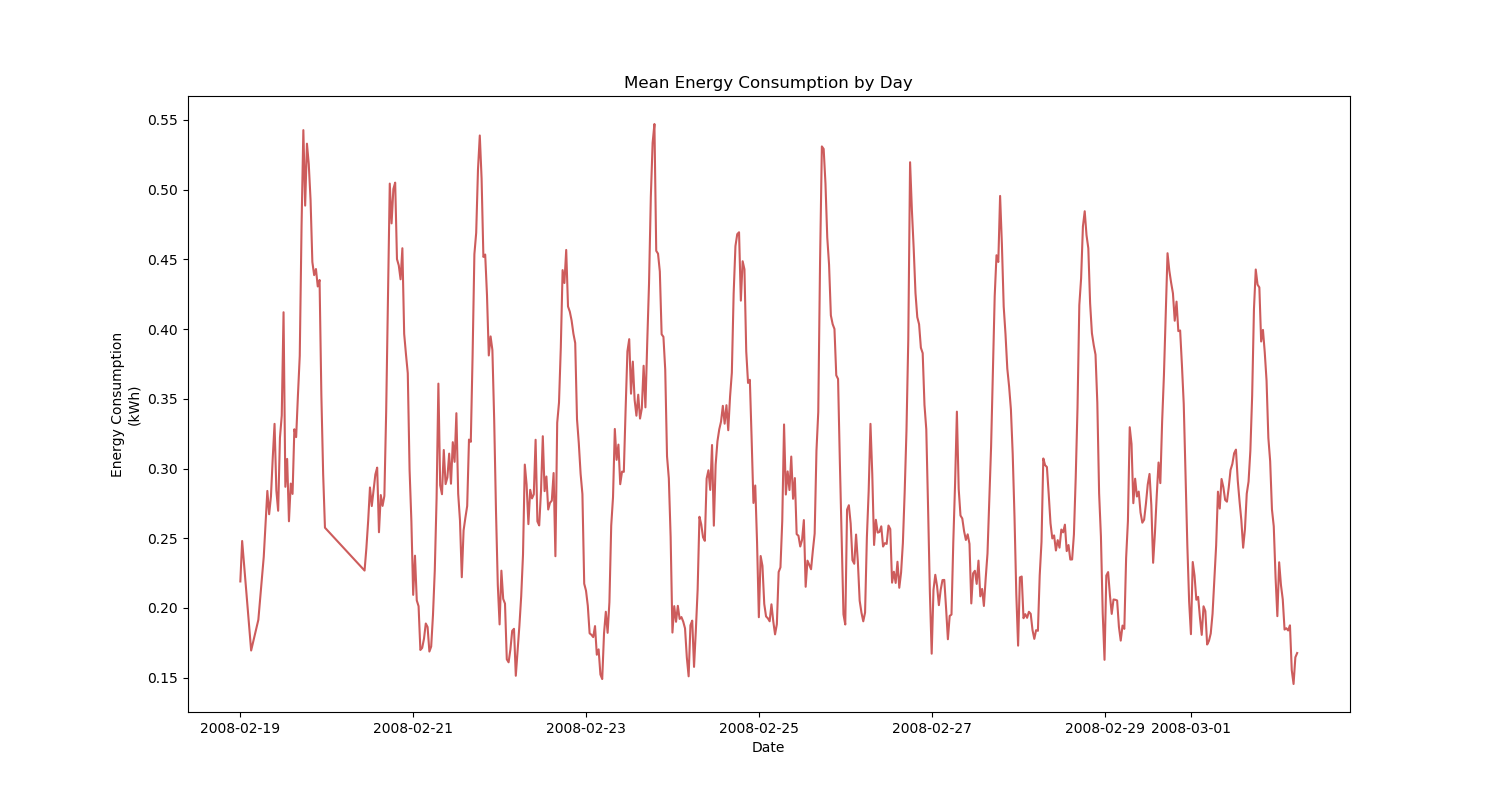
\includegraphics[width=1\textwidth]{Figures/EDA_images/mean_consumption_day.png}
        \caption{Mean Consumption for All Meters}
        \label{fig:Mean Consumption}
        \end{figure} 
        
        Figure 3.1 shows the mean consumption of energy across all devices for 12 day period.  Here we can see the huge variation in load on a daily basis. There appears to be a clear daily trend with a peak at some point during the day, a low point at some point and a period of medium energy consumption in between. To further investigate the daily cycle of energy consumption, fig.3.2. shows the mean energy consumption of a 24 hour period on a half-hourly resolution from the data set. Here we see the period between midnight and 5am has the lowest half-hour energy consumption with approx 0.2kWH consumed every 30 minutes per smart meter. This has significant importance to energy providers as this corresponds to the minimum amount of energy that has to be produced 24/7. After 5am a step incline in energy consumption can be observed, from 0.2 kWH to 0.3 kWh, which then holds consistently until approx 3pm. After 3pm we again see a further step incline to a peak of ~0.48 kWh just before 8pm before falling off dramatically.
        
        \begin{figure}[H]
        \centering     
        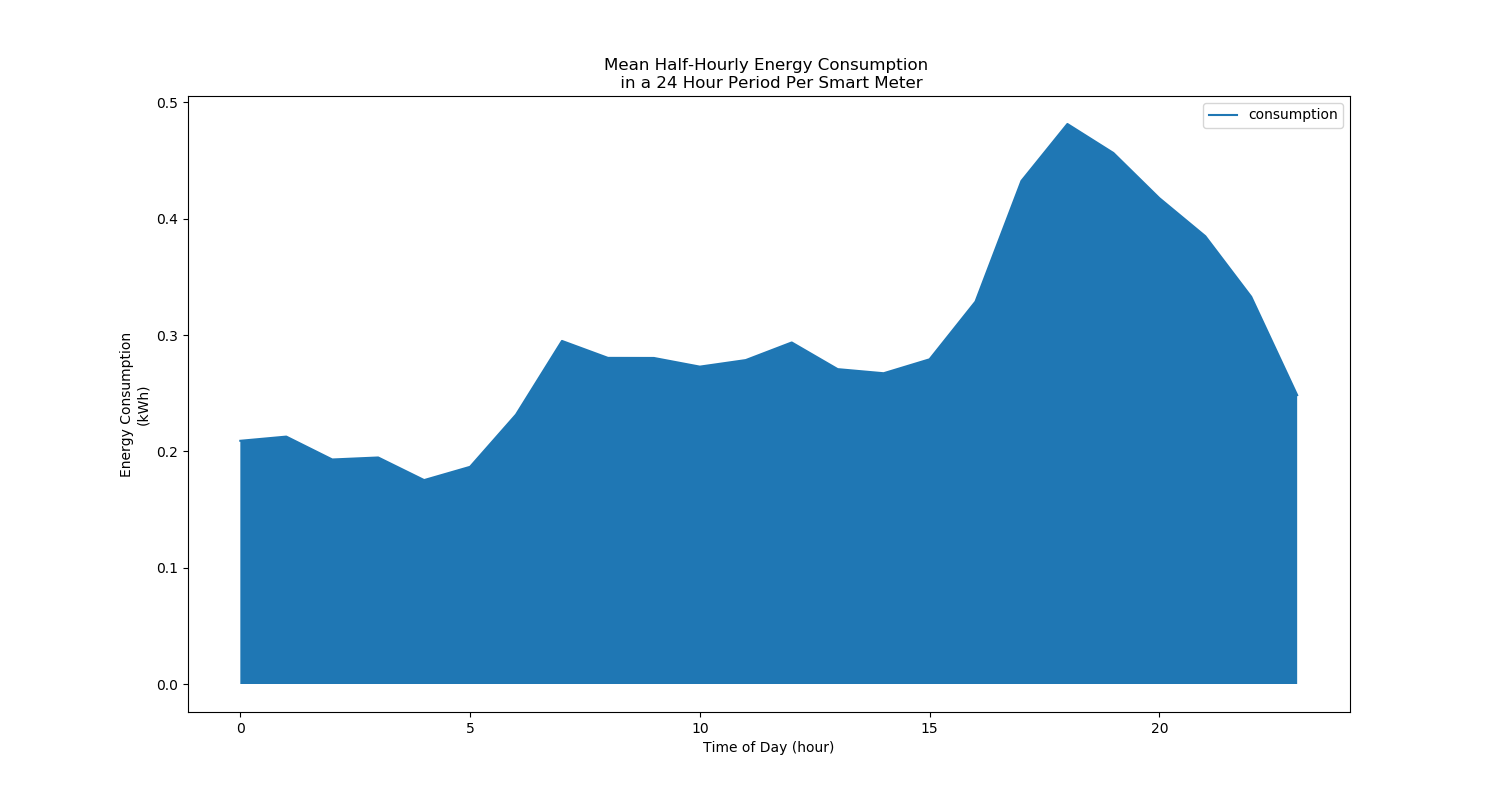
\includegraphics[width=1\textwidth]{Figures/EDA_images/mean_consumption_one_day.png}
        \caption{Mean Consumption per 24 Hour Period Per Smart Meter}
        \label{fig:Daily Consumption}
        \end{figure}
        
        Apart from looking at energy consumption values per time period, we can also investigate consumption values for the unique smart meter ANON\_IDs. In fig.3.3. we see the histogram generated to represent the frequency of mean energy consumption per half-hour per smart meter. This 'chunk' of data contains 295 unique ANON\_IDs, the mean half-hourly energy consumption is 0.281 kWh compare that to the median value of 0.250 kWh backup up the observed positive skew. The minimum is 0.0265 kWh compared the maximum value of 1.385 kWh representing a range of 1.3585 kWh. Fig.3.4. shows a box plot of the mean energy consumption per 30 minute interval per device. Here we there is an interquartile range (IQR) of 0.1965 kWh (0.1534 to 0.35 kWh). We can also observe a number of potential outliers above the $Q_3 + 1.5IQR$ value represented by the whisker.
        
        \begin{figure}[H]
        \centering     
        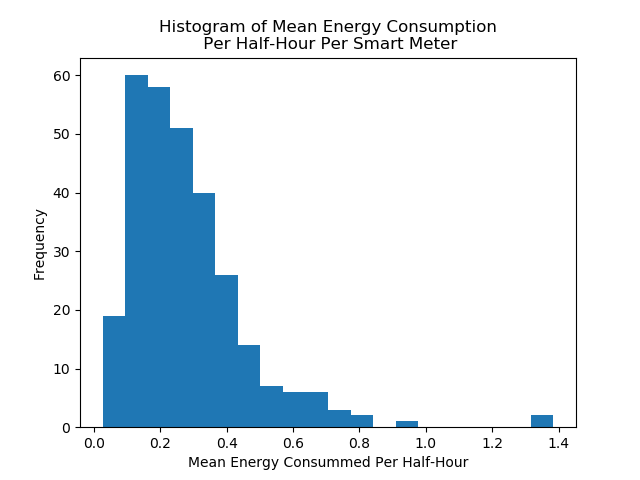
\includegraphics[width=1\textwidth]{Figures/EDA_images/mean_consumption_histogram.png}
        \caption{Histogram of Mean Consumption by ANON\_ID}
        \label{fig:Daily Consumption}
        \end{figure}
        
        \begin{figure}[H]
        \centering     
        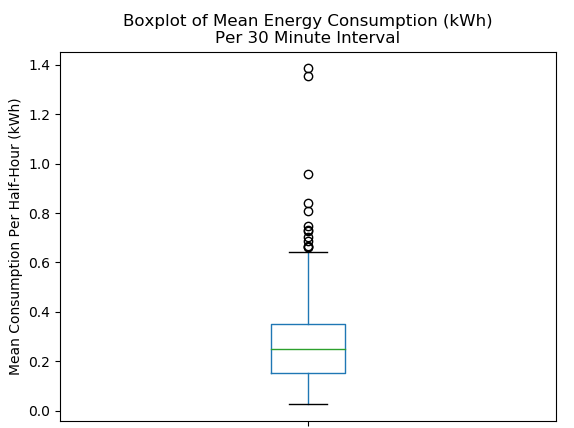
\includegraphics[width=0.75\textwidth]{Figures/EDA_images/mean_consumption_boxplot.png}
        \caption{Boxplot of Mean Consumption by ANON\_ID}
        \label{fig:Daily Consumption}
        \end{figure}
        
        These outliers may be indicative of a potential cluster, the distribution fig.3.3. shows that we have a narrow distribution, the standard distribution of the sample is 0.1827 kWh. If we were to translate that to clustering based on mean energy consumption we could expect to see a large cluster of low energy consumption dwellings with a centroid close to the median, a comparatively lower number of medium energy with a centroid approximately in the 0.5 to 0.8 kWh range and a third cluster with high energy usage. This outlines a point made in section 2.3.1. on limitations of k-means clustering which expects clusters of equal or similar size.
        
        \subsection{LAD 2011 UK Names and Codes} \\
        This data set contains Local Authority Districts (LAD) names and codes.
        
        \subsection{Geographic Data}
        \subsubsection{Description of Variables}
        \\
        This file is in XLSX format. This data set contains geographic data (Government Office Region and Local Authority) and ACORN segmentation data which can be linked to the consumption data via an anonymised household ID. ACORN is a segmentation tool which categorises the UK's population into demographic types. ACORN segments households, postcodes and neighbourhoods into 6 categories, 18 groups and 62 types. The following table outlines the variables contained within the Geographies data set:
        
        \begin{center}
            \begin{tabular}{|l |l|}
            \hline
             \textbf{Variable Name} & \textbf{Description} \\
             \hline\hline
             ANON\_ID & Integer case identifier (unique, not null, \\& use to link records in the other files) \\ 
             \hline
             eProfileClass & Domestic electricity profile class (1 or 2) \\
             \hline
             fuelTypes & Fuel Type - ElecOnly, GasOnly, or dual \\
             \hline
             ACORN\_Category & CACI Acorn category value \\
             \hline
             ACORN\_Group & CACI Acorn group value \\
             \hline
             ACORN\_Type & CACI Acorn type value \\
             \hline
             ACORN\_Code & CACI Acorn category, group and type values in one string \\
             \hline
             ACORN\_Description & English language description of CACI Acorn code \\
             \hline
             NUTS4 & Reflects the LAU1 areas to UK administrative \\&  geographies from 1$^{st}$ April 2010 \\
             \hline
             LACode & Reflects the UK Local Authority  boundaries that \\&  were in place on 21$^{st}$ June 2010\\
             \hline
             NUTS1 & Reflects the 12 NUTS1 areas to UK administrative \\& geographies from 1$^{st}$ April 2010\\
             \hline
             gspGroup & Electricity transmission network Grid Supply \\& Point Group code\\
             \hline
             LDZ & Gas transmission network Local Distribution Zone code\\
             \hline
             ELEC\_TOUT & Households containing an electricity meter \\& with a time of use tariff\\
             \hline
             GAS\_OUT & Households containing a gas meter with a time of use tariff\\
             \hline
            \end{tabular}
        \end{center}
        
        \subsubsection{Exploratory Data Analysis on Geographic Data Set}
        
        \begin{figure}[H]
        \centering     
        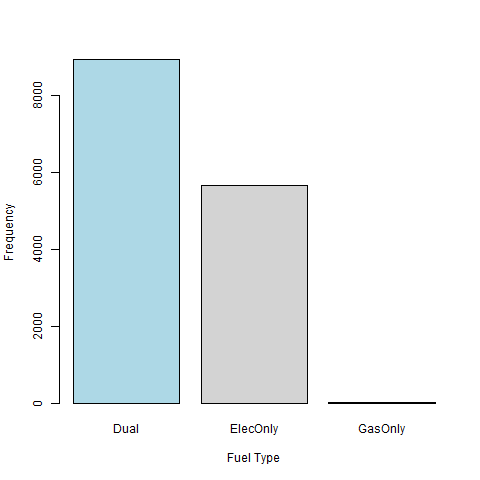
\includegraphics[width=1\textwidth]{Figures/EDA_images/fuel_table.png}
        \caption{Histogram of Mean Consumption by ANON\_ID}
        \label{fig:Daily Consumption}
        \end{figure}
        
        \begin{figure}[H]
        \centering     
        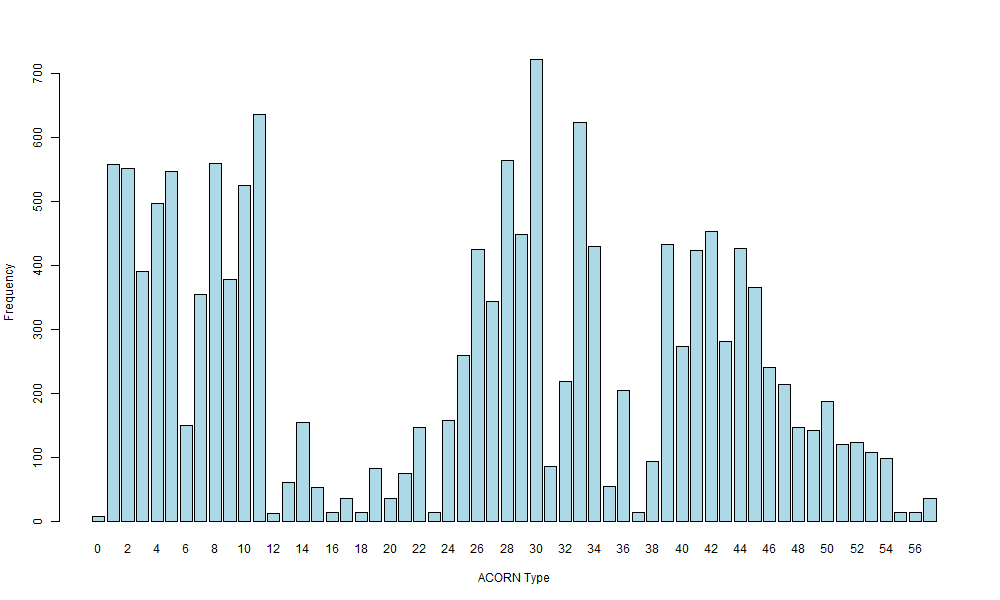
\includegraphics[width=1\textwidth]{Figures/EDA_images/acorn_type.png}
        \caption{Histogram of Mean Consumption by ANON\_ID}
        \label{fig:Daily Consumption}
        \end{figure}
        
        \begin{figure}[H]
        \centering     
        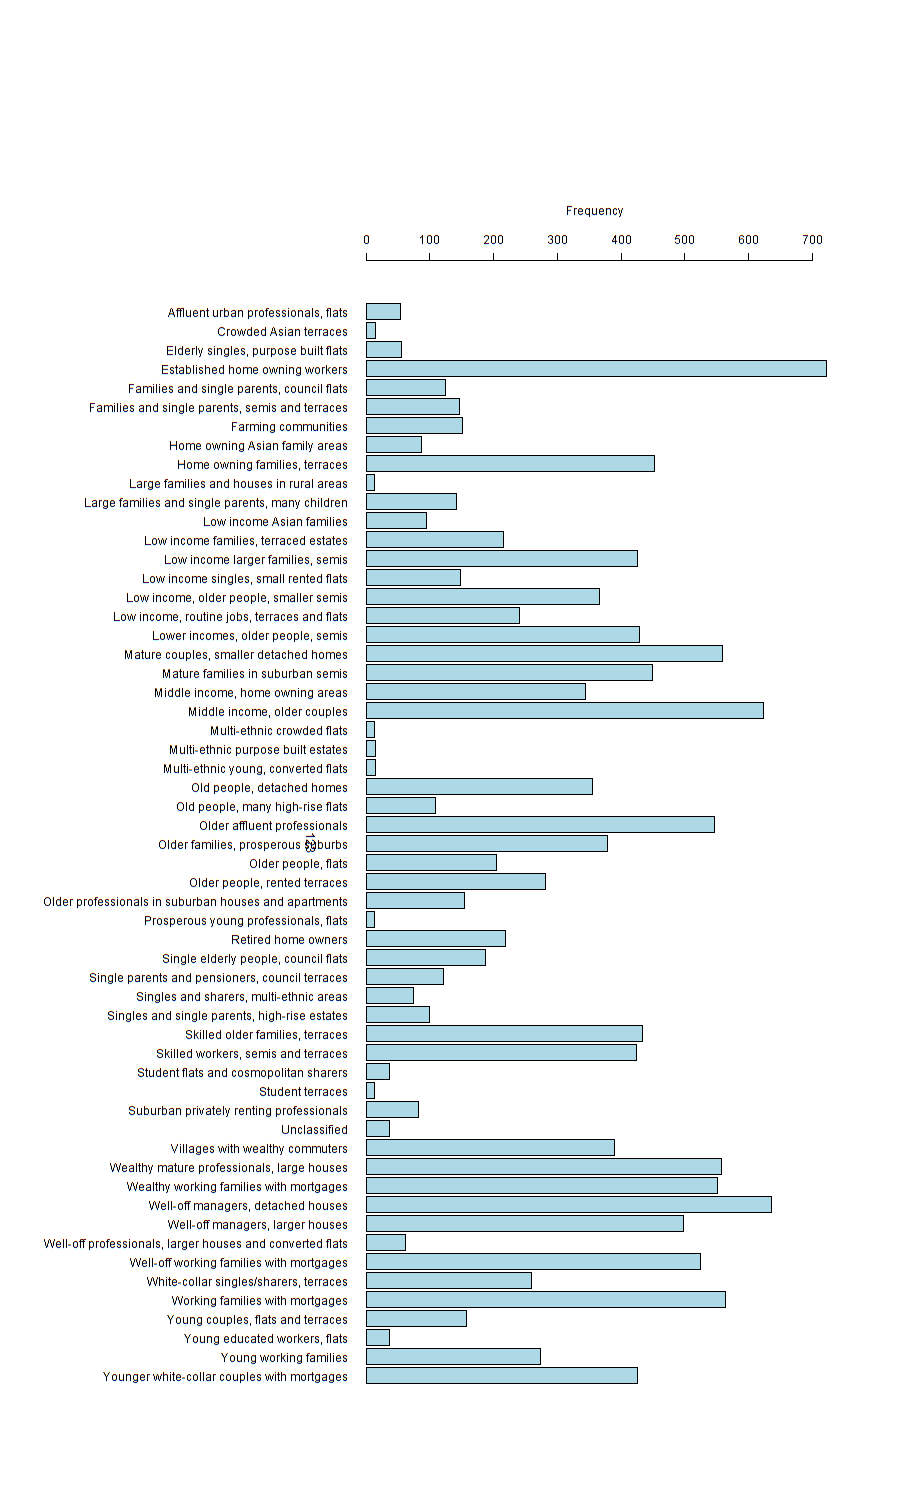
\includegraphics[width=1\textwidth]{Figures/EDA_images/acorn_description.png}
        \caption{Histogram of Mean Consumption by ANON\_ID}
        \label{fig:Daily Consumption}
        \end{figure}
        
        \subsection{Metadata} \\
        The metadata data set is a file containing explanatory descriptions of variables:
        
        \begin{left}
            \begin{tabular}{| l | l |}
            \hline
             \textbf{Variable Name} & \textbf{Description} \\
             \hline\hline
             Hhold\_ID & Integer case identifier (unique, not null, \\& use to link records in the other files) \\ 
             \hline
             firstAdvance & Date-Time of earliest electricity advance (halfhour
             precision) \\
             \hline
             fuelTypes & Fuel Type - ElecOnly, GasOnly, or dual \\
             \hline
             lastAdvance & Date-Time of latest electricity advance (halfhour
             precision) \\
             \hline
             days\_in\_range & Inclusive number of days between firstAdvance and
             lastAdvance \\
             \hline
             minAdvance & Lowest electricity advance value \\
             \hline
             maxAdvance & Highest electricity advance value \\
             \hline
             meanAdvance & Average electricity advance value \\
             \hline
             n\_expected & Number of advances expected based on
             days\_in\_range \\
             \hline
             n\_found & Number of advances available\\
             \hline
             pctFound & n\_expected/n\_found\\
             \hline
             TOUT & Time-of-use identifier\\
             \hline
            \end{tabular}
        \end{left}
        
        \subsection{Accompanying Documentation}\\
        PDF document containing all descriptions of data sets and variables contained within.
\section{Description of Process}
    In this section the workflow is described in detail and the challenges are outlined and discussed. It is as follows:
    \begin{itemize}
        \item Working With Large Data Sets
        \item Time Series and Dataframe Structure
        \item Clustering Time Series Data
        \item Pre-Process Geographic Data Set
        \item Build \& Tune The Random Forest Model
    \end{itemize}
    
\begin{figure}[H]
\centering     
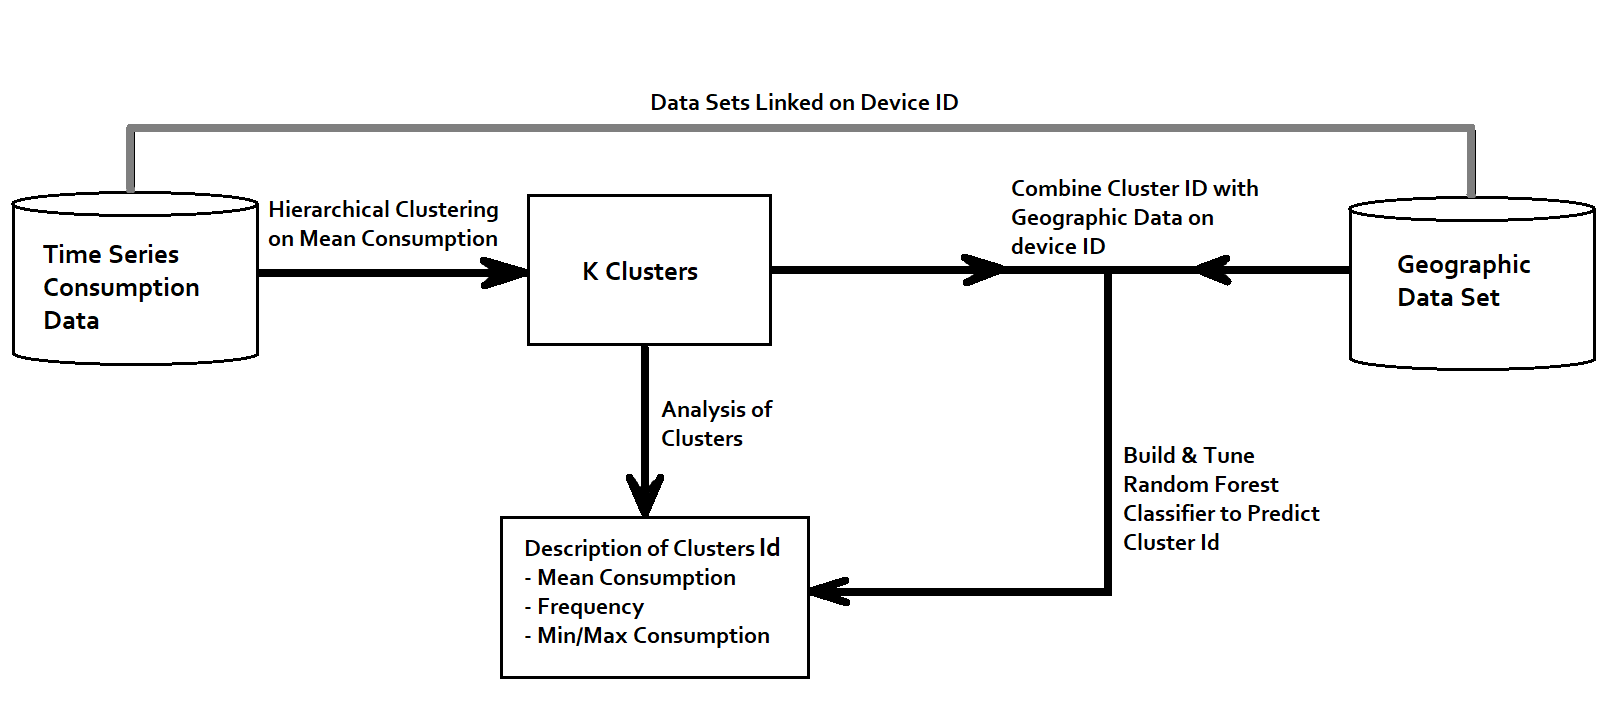
\includegraphics[width=1\textwidth]{Figures/workflow.png}
\caption{Work Flow of Project}
\label{fig:Dendrogram}
\end{figure} 
    
    \subsection{Working With Large Data Sets}
    As mentioned in section 3.1, the CSV file containing the half-hourly electrical energy consumption readings is 12GB in size. Reading this file into memory would likely cause a system failure due to the size of the file and limitations in RAM capacities. This is a common problem in working with Big Data and there are novel solutions available rather than just adding more RAM to the system. Some data sets can be terabytes in size so scaling up RAM isn't always cost efficient or even possible, a different approach this problem would be to read the file into memory in chunks. This would allow for a manageable portion of the data set to be read into memory, analysed and then dropped from memory, freeing up space for the next chunk and repeating this process until the entire data set has been processed. This would allow for a data set with $n$ number of observations to be partitioned into $k(\leq n)$ chunks such that $C = \{C_1, C_2, \dots, C_k\}$ (where each observation is assigned to one chunk) as to maximize the available memory limit. Maximizing the size of $k$ while not hitting the upper memory threshold would allow for shorter compute times as the number of iterations is inversely proportional to $k$. Another benefit to using this approach would be utilizing a distributed computing system. By breaking the data set down into chunks, the task of processing each one can be divided out into a number of different systems such that chunk $C_1$ is sent to system $S_1$, chunk $C_2$ sent to system $S_2$ and so forth. By working on the problem in parallel, the time taken to process the overall data set is reduced.
    
    \subsection{Time Series and Dataframe Structure}
    The original electrical consumption data set as mentioned in 3.1.1 is ordered by ADVANCEDATETIME. When this is partitioned into chunks, there is no prior knowledge of what ANON\_ID are contained within that chunk. The dataframe should be structured where each column is series of all the consumption values for a ANON\_ID. To do this, the chunk is looped through, new ANON\_IDs are identified and consumption values are appended to the corresponding ANON\_ID column and date-time row. The following table shows the final structure of the time series data for a chunk containing $j$ number of unique ANON\_IDs, $i$ number of date-time stamps ($t$) and energy consumption values $V$. Note that not all ANON\_IDs will be of the same length so there will be null values.

% HERE: TABLE DISPLAYING STRUCTURE OF TIME SERIES DATA FRAME    
\[ \begin{array}{l | cccccl}
\mbox{}         & anon\_id_1    & anon\_id_2    & anon\_id_3    & \quad ...     & \quad \rightarrow   & anon\_id_j \\
\hline
\mbox{t$_1$}    & V_{1,1}       &  V_{1,2}      &  V_{1,3}      & \quad ...     & \quad\rightarrow    &  V_{1,j}   \\
\mbox{t$_2$}    & V_{2,1}       &  V_{2,2}      &  V_{2,3}      &               &           & \\
\mbox{t$_3$}    & V_{3,1}       &  V_{3,2}      &  V_{3,3}      &               &           & \\
\mbox{...}      & ...           &               &               &\quad ...      &           & \\
\downarrow      & \downarrow    &               &               &               & \searrow  & \\
\mbox{t$_i$}    & V_{i,1}       &               &               &               &           & V_{i,j} \end{array}\]
    
    \subsection{Clustering Time Series Data}
    Now that the dataframe is in the correct structure, the time series data can be clustered. For clustering the SciPy library was imported, in order to perform hierarchical clustering the scipy.cluster.hierarchy.linkage() function was used. This function takes an input $y$ which may be in the form of a 1D condensed distance matrix or a 2D array of observation vectors, the latter is passed in. The following linkage methods are used to compute the distance $d(s,t)$ between two clusters $s$ and $t$. The algorithm begins with a forest of clusters that have yet to be used in the hierarchy being formed. When two clusters $s$ and $t$ from this forest are combined into a single cluster $u$, $s$ and $t$ are removed from the forest, and $u$ is added to the forest. When only one cluster remains in the forest, the algorithm stops, and this cluster becomes the root.
    
    A distance matrix is maintained at each iteration. The d[$i,j$] entry corresponds to the distance between cluster $i$ and $j$ in the original forest.

    At each iteration, the algorithm must update the distance matrix to reflect the distance of the newly formed cluster u with the remaining clusters in the forest.
    
    Suppose there are $|u|$ original observations $u[0],\dots, u[|u| -1]$ in cluster $u$ and $|u|$ original objects $v[0], \dots, v[|v| -1]$ in cluster $v$. Recall $s$ and $t$ are combined to form cluster $u$. Let $v$ be any remaining cluster in the forest that is not $u$.
    
    The following are method is used for calculating the distance between the newly formed cluster $u$ and each $v$.
    
    \begin{equation}
d(u, v) = \sum_{ij} \frac{d(u[i], v[j])}{(|u| \times |v|)}
    \end{equation}\
    
    For all points $i$ and $j$ where $|u|$ and $|v|$ are the cardinalities of clusters $u$ and $v$, respectively. This is also called the UPGMA algorithm.
    
    The metric used to calculate the distance was discussed in section 2.3.3
    
    The scipy.cluster.hierarchy.fcluster() function is used to form flat clusters from the hierarchical clustering defined by the linkage matrix. The hierarchical clustering encoded with the matrix returned by the linkage function is passed into the function. The maximum number of clusters..
    All the ANON\_IDs in the chunk are assigned a cluster.
    
    % PREPROCESSING THE GEO DATA (INCLUDING CHECKING NAs)
    \subsection{Pre-processing The Geographic Data}
    The geographic data set will be used in combination with the results of the clustering process in order to build an RF model capable of classifying a domestic energy consumer's energy needs. Before we build the classifier, the existing geographic data must be pre-processed in order to improve the accuracy of the model.
    Firstly some of the variables are removed, ACORN\_Category, ACORN\_Group, ACORN\_Description and ANON\_ID either fall under the category of indicator variables or variables that are directly correlated to other variables and therefore these variables are removed. 
    
     % dummy variables
    Next the remaining variables are converted to dummy variables. A dummy variable takes on the values of 0 or 1 to indicated the absence or presence of some categorical effect that may be expected to shift the outcome, note this increases the number of variables from 10 to 304. The R Library called '\textit{Caret}' will be utilized to carry out further pre-processing. The caret package(short for Classification And REgression Training) contains functions to streamline the model training process for complex regression and classification problems. Using caret we're going to remove near-zero variance variables. These are variables which either have a single unique value or unique value that occur with very low frequencies, for a model such as random forest it can cause them to become unstable so we're going to remove them here. This reduced the dimension of the data set down from (14,621 $\times$ 304) to (14,621 $\times$ 28), a considerable drop in variables.
    
    % remove correlated features
    Next we're going to look at correlated explanatory variables. To do this we make a correlation matrix, we can see that there were 2 variables with almost perfect correlation. Before we remove the variables, we use descrCor to get an idea of the overall correlation, it shows an overall mean correlation of -0.01823. We next set a cut-off of 0.75 and remove any variables with a correlation higher than this. This drops the dimension of the data down to (14,621 $\times$ 15), however the overall mean correlation is now -0.03837 which is marginally higher. Despite the marginal increase in correlation, the removed correlated features are not added back into the data set, here we are favoring a reduced complexity model. Note we also checked the data for linear dependencies and found none.
    % centre and scale
    Now we can center and scale the data. To do this we use the preProcess() function provided in \textit{Caret}. The final steps are to add back the ANON\_ID which we removed in the beginning. We also will map the results of the clustering onto the ANON\_ID.
    
    
    \subsection{Build and Tune Classification Models}
    In this section we will build 3 different models on the pre-processed data sets. There models will be used to predict what mean energy consumption cluster a consumer belongs to. The 3 models we will build are the Random Forest Model (RF), Gradient Boosting Model (GBM) and Support Vector Machine Model (SVM).
    
    For each models we will automate the tuning process using the \textit{Caret} library. To do this we first setup the training/test split in order to evaluate the models for the tuning process. Here we chose a 25-75 split. To evaluate the models we us a cross-validation technique in order to reduce the variance between models. Additionally we don't specifically want to choose the model with the highest accuracy as that model may be over fitting. To implement Occam's razor into our evaluation process we are going to define our selection function to chose the model within 2\% of the best model with the \textit{simplest parameters}. The evaluation metric is going to be based on the accuracy of the model.
    
    \subsubsection{Random Forest Model}
    The tuning parameters for the RF model are as follows:
        % list tuning parameters
        \begin{center}
            \begin{tabular}{|l |l|}
            \hline
             \textbf{Parameter} & \textbf{Chosen Values} \\
             \hline\hline
             mtry & $\sqrt{n}$ where n = number of features in train set \\
             \hline
            \end{tabular}
        \end{center}
    
    \subsubsection{Gradient Boosting Model}
    The tuning parameters for the GBM model are as follows:
        % list tuning parameters
        \begin{center}
            \begin{tabular}{|l |l|}
            \hline
             \textbf{Parameter} & \textbf{Chosen Values} \\
             \hline\hline
             Interaction Depth & [1, 5. 9] \\
             \hline
             N.trees & 50 - 1,500 in steps of 50 \\
             \hline
             shrinkage & Held constant at 0.1 \\ 
             \hline
             n.minobsinnode & Held constant at 20 \\
             \hline
            \end{tabular}
        \end{center}
        
        \subsubsection{Support Vector Machine Model}
        The tuning parameters for the SVM model are as follows:
        % list tuning parameters
        \begin{center}
            \begin{tabular}{|l |l|}
            \hline
             \textbf{Parameter} & \textbf{Chosen Values} \\
             \hline\hline
             preProc & [center, scale] \\
             \hline
             Tune Length & Held constant at 8\\
             \hline
            \end{tabular}
        \end{center}